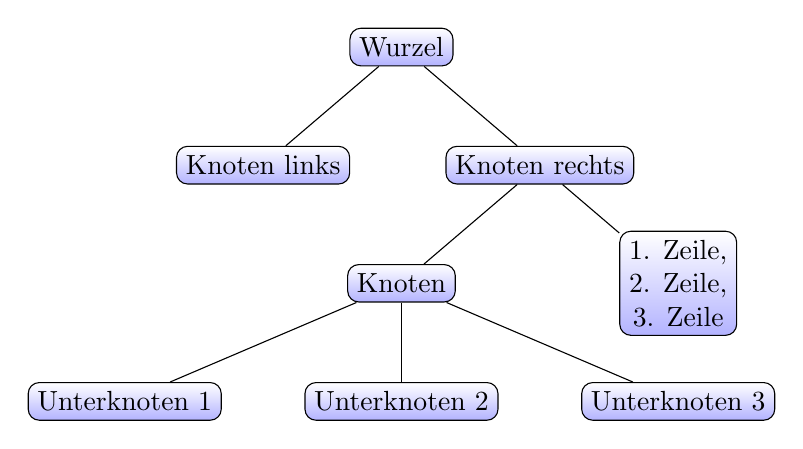
\begin{tikzpicture}[sibling distance=10em,
  every node/.style = 
  	{shape=rectangle, rounded corners,
    draw, align=center,
    top color=white, bottom color=blue!30}
]
    
  \node {Wurzel}
    child { node {Knoten links} }
    child { node {Knoten rechts}
      child { node {Knoten}
        child { node {Unterknoten 1} }
        child { node {Unterknoten 2} }
        child { node {Unterknoten 3} } }
      child { node {1. Zeile,\\2. Zeile,\\3. Zeile} } };

\end{tikzpicture}